Přehled současného stavu se věnuje základnímu anatomickému popisu srdce společně
s úvodem do jeho fyziologie a elektrofyziologie ve spojení s neurofyziologickými
vlivy. Dále jsou zde popsány principy vyšetřovacích metod v kardiologii,
konkrétně oblast měření, zpracování a analýza elektrického záznamu srdeční
aktivity. Závěr kapitoly je věnován detailnějšímu rozboru variability srdeční
frekvence (HRV), která je předmětem analýzy zpracovaného EKG záznamu v rámci
této práce.

\subsection{Srdce}
\label{section:heart}
Srdce (cor) je orgán nepravidelného kuželovitého tvaru velkého zhruba jako pěst
dospělého člověka, skládající se převážně ze svaloviny \cite{Memorix2017}. Tato
pravidelně oscilující pumpa zastupuje v kardiovaskulárním systému funkci
krevního čerpadla a umožňuje tak setrvalý běh organismu. Nachází se ve střední
částí hrudní dutiny (cavitas thoracica) mezi pravou a levou pleurální blánou
(pleura mediastinalis dextra et sinistra) v prostoru za sternem nazývaném
mediastinum. \cite{Weinhaus2005}.

\begin{figure}[h]
	\begin{center}
		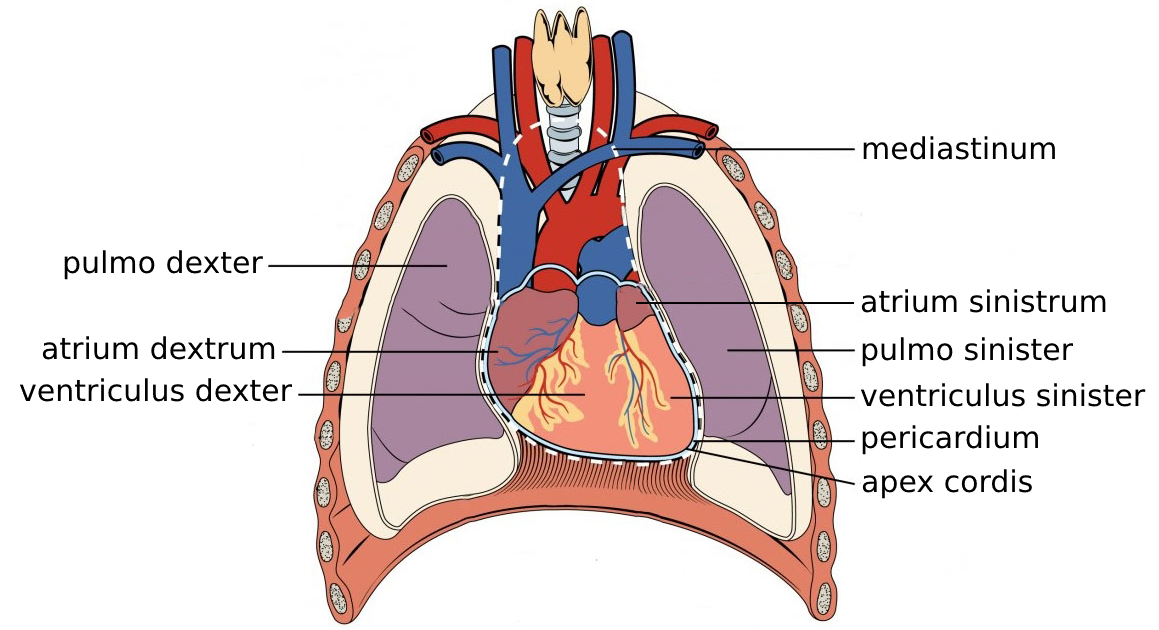
\includegraphics[width=0.7\textwidth]{../assets/anatomy/mediastinum}
		\caption{Umístění srdce v hrudní dutině mezi plícemi v mediastinu
			(Upraveno a převzato z \cite{OpenStax})}
		\label{fig:mediastinum}
	\end{center}
\end{figure}

\subsubsection{Struktura srdce}
\label{section:heart_structure}
Vnitřní svalová struktura srdce je tvořena dvěma síněmi (atrium dextrum et
sinistrum) a dvěma komorami (ventriculus dexter et sinister), oddělenými
mezikomorovou přepážkou (septum interventriculare), která současně rozděluje
srdce na levé a pravé \cite{Memorix2017}. O tok krve srdcem se starají čtyři
srdeční chlopně, fungující jako jednosměrné ventily, které jsou vidět na Obr.
\ref{fig:heartanatomy}, přičemž z komory pravého srdce je přečerpávána
neokysličená krev do plic. Z komory levého srdce se pumpuje okysličená krev do
celého krevního oběhu, a proto je svalovina levé komory silnější. Rozdíl zde
není jen ve svalovině ale také v krevním tlaku, jelikož pumpování krve do
tělního oběhu vyžaduje mnohem větší tlak než do plicního oběhu. Rozlišujeme tedy
malý a velký oběh neboli krevní cirkulaci pulmonální a systémovou. Systematicky
k této cirkulaci dochází díky řetězci opakujících se elektrických a mechanických
událostí, uskutečněných během jedné časové periody, nazývané srdeční cyklus
(srdeční revoluce). Konkrétně se jedná o svalovou kontrakci (systola) a svalovou
relaxaci (diastola). Blíže je tento cyklus popsán v kapitole
\ref{section:cardiac_cycle}. Průtok krve srdcem je znázorněn pomocí bílých šipek
na ilustraci níže \cite{Stejfa2006}.

\begin{figure}[h]
	\begin{center}
		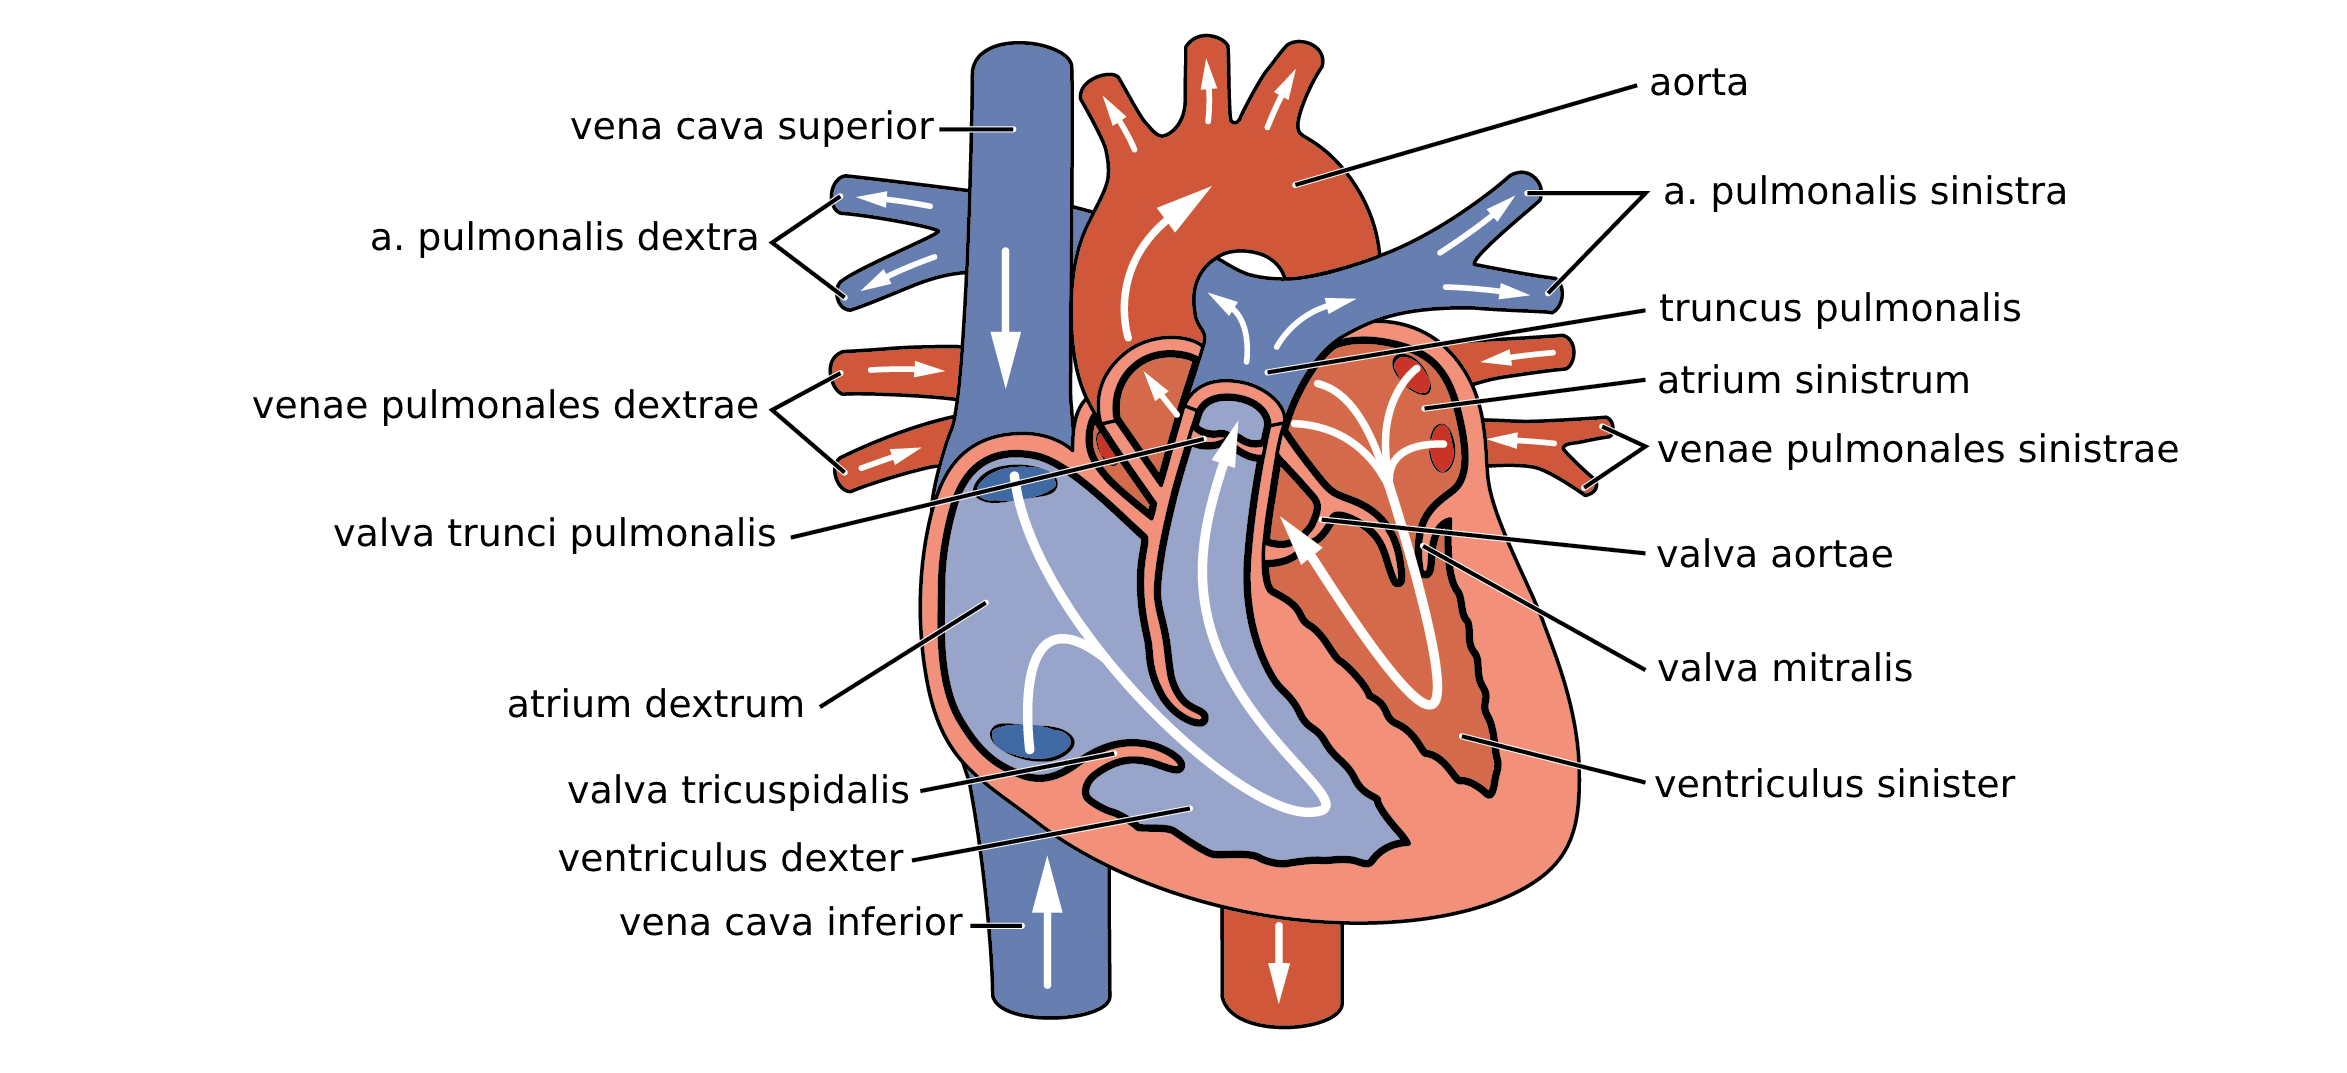
\includegraphics[width=1\textwidth]{../assets/anatomy/heart}
		\caption{Schéma srdce (anteriorní řez) zobrazující tok krve srdcem
			prostřednictvím bílých šipek (Upraveno a převzato z
			\cite{OpenStax})}
		\label{fig:heartanatomy}
	\end{center}
\end{figure}

Vnější svalovina, obdobně jako u cév, sestává ze tří vrstev: myokard (tunica
media), endokard (tunica intima) a epikard (tunica serosa), které společně tvoří
mohutný segment srdeční stěny \cite{Memorix2017}. Myokard (myocardium), nejširší
část srdeční stěny podléhající kontrakcím, je tvořen v závislosti na srdečním
oddílu dvěma až třemi vrstvami příčně pruhované svaloviny. Na myokard naléhá
silná řídká vrstva kolagenního vaziva a tuku neboli epikard (epicardium), ve
které probíhají cévy zásobující srdce. Poslední vrstvou, která vystýlá srdeční
dutiny a mezi síněmi a komorami tvoří mitrální chlopně, je endokrad
(endocardium). Povrch srdce obaluje vnitřní vazivový list, epikard (epicardium),
který podél vnějších srdečních cév přechází do vazivově-serózní blány,
osrdečníku (pericardium). Perikard zabraňuje krevnímu přeplnění srdce a
přetíženosti srdeční svaloviny. Prostor mezi perikardem a epikardem je vyplněn
malým množstvím serózní tekutiny, umožňující jejich vzájemný klouzavý pohyb, a
nazývá se perikardiální dutina (cavitas pericardialis)
\cite{Weinhaus2005,Dylevsky2013}.

\begin{figure}[h]
	\begin{center}
		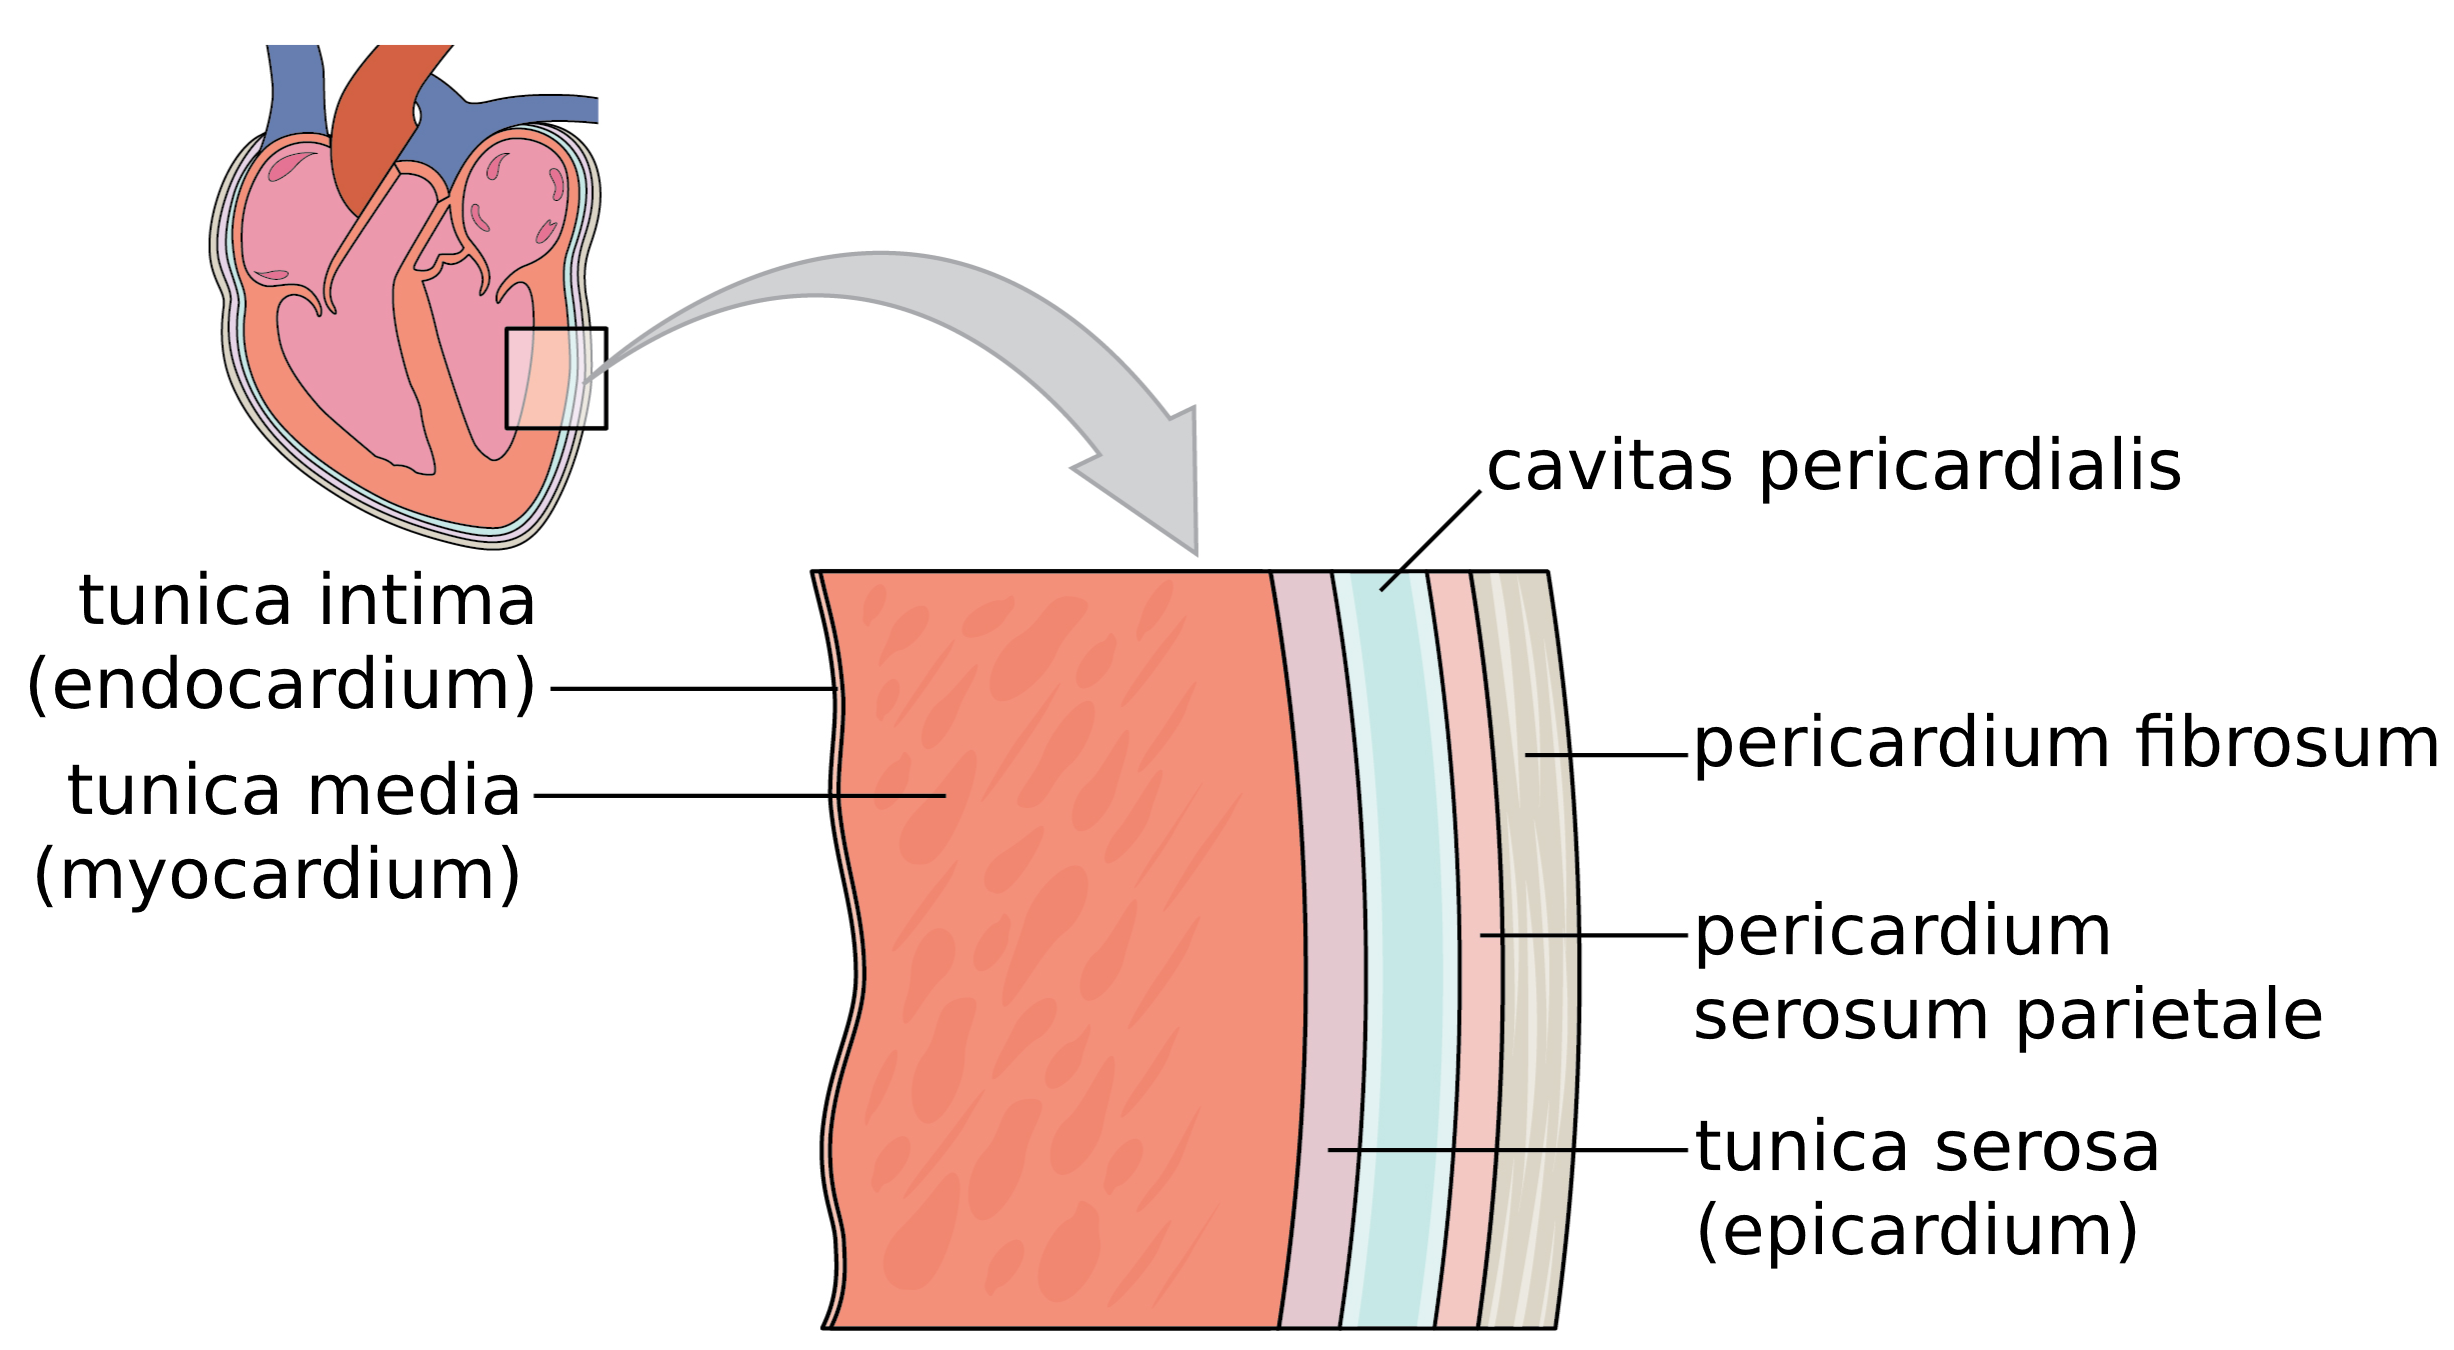
\includegraphics[width=0.6\textwidth]{../assets/anatomy/heart_muscle}
		\caption{Perikardiální membrána a vrstvy srdeční stěny (Upraveno a
			převzato z \cite{OpenStax})}
		\label{fig:heartlayers}
	\end{center}
\end{figure}

Obecně se srdeční svalovina skládá z příčně pruhované srdeční tkáně, kombinující
vlastnosti kosterního a hladkého svalstva, avšak k zajištění srdeční činnosti
obsahuje kromě svalových buněk schopných kontrakce (pracovní myokard) také
specializované kardiomyocyty, tvořící převodní systém srdeční (PSS). Tento
systém společně ve spojení s autonomním nervovým systémem (ANS) tvoří pro tuto
práci zásadní část, a proto je podrobněji probrán v samostatné kapitole
\cite{Memorix2017,Dylevsky2013}.

\subsubsection{Srdeční cyklus}
\label{section:cardiac_cycle}
Jak již bylo naznačeno v kapitole \ref{section:heart_structure}, dvě z hlavních
funkcí srdce jsou: přečerpat neokysličenou krev ze systémového oběhu do plic,
kde dojde k její oxygenaci a pumpovat okysličenou krev z plic zpět do všech
tkání, kde dojde znovu k její deoxygenaci a celý proces se tak znovu opakuje.
Srdeční cyklus je tedy časově sladěný průběh dvou hlavních fází začínající
systolou a končící diastolou \cite{Weinhaus2005}. Systola je okamžik, kdy je ze
srdce kontrakcí a za vysokého tlaku vypuzována krev do oběhu, zatímco při
diastole neboli plnící nízkotlaké fází, se srdce krví plní. Síně i komory
podléhají oběma těmto fázím a jsou koordinovány otvíráním a zavíráním
atrioventrikulárních a semilunárních chlopní. Zároveň je regulována i čerpací
funkce srdce, tak aby v každém momentu byly splněny nároky tkání na okysličenou
krev \cite{OpenStax}. Detailněji jsou jednotlivé fáze srdečního cyklu popsány
níže.

\begin{figure}[h]
	\begin{center}
		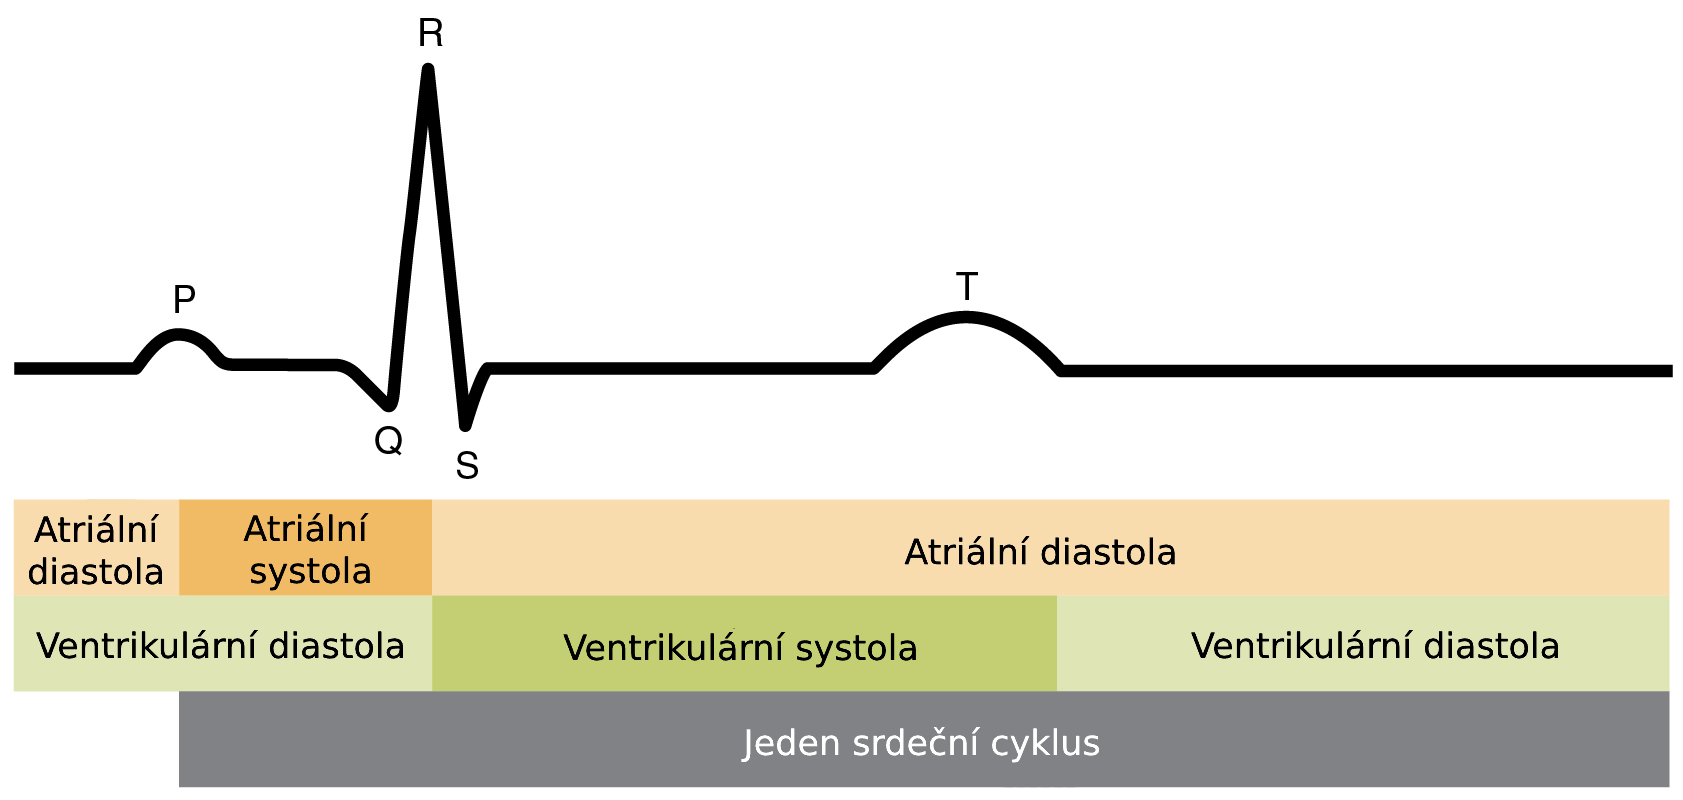
\includegraphics[width=0.8\textwidth]{../assets/anatomy/cardiac_cycle_ecg}
		\caption{Vztah mezi srdečním cyklem a EKG (Upraveno a převzato z
			\cite{OpenStax})}
		\label{fig:cardiac_cycle_ecg}
	\end{center}
\end{figure}

\paragraph*{\textit{Plnící fáze (atriální diastola)}\\} Síně a komory jsou
relaxované. Komory srdce se pod nízkým tlakem (0--10 \si\mmHg) plní
neokysličenou krví přicházející ze systémového oběhu. Krev proudí do levé síně z
venae cave inferior et superior a sinus coronarius. Do lévé síně přichází krev z
plicních žil. Otevřenou trikuspidalní a mitrální chlopní proudí krev dál ze síní
právě do komor. Komory se naplní krví přibližně do 70--80 \% jejich kapacity
\cite{OpenStax}.

\paragraph*{\textit{Izovolumická fáze (atriální systola)}\\} Síně podléhají
kontrakci a zvyšuje se v nich tlak (80--120 \si\mmHg). Díky tomu je do komor
otevřenými atrioventrikulárními chlopněmi dopraveno zbylých 20--30 \% krve.
Kontrakce síní je zároveň doprovázená depolarizací, kterou na EKG reprezentuje P
vlna a trvá přibližně 100 \si\ms. Konec fáze je doprovázen otevřením
semilunárních chlopní \cite{OpenStax}.

\paragraph*{\textit{Ejekční fáze (ventrikulární systola)}\\} Tlak v komorách
roste následkem jejich kontrakce, dokud není dostatečně velký, aby došlo k
otevření semilunárních chlopní. Krev je pak vypuzena z komor do tepen, přičemž v
komorách vždy zůstává konečný systolický objem (end systolic volume, ESV) krve,
který činí přibližně 50--60 \si\ms. Ventrikulární systola je doprovázena
depolarizací komor, která je na EKG záznamu reprezentovaná jako QRS komplex.
Tato fáze trvá přibližně 270 \si\ms \cite{OpenStax}.

\paragraph*{\textit{Fáze izovolumické relaxace (ventrikulární diastola)}\\}
Ventrikulární relaxace je doprovázená repolarizací komor a na EKG reprezentovaná
T vlnou. Trvá přibližně 430 \si\ms. Komory přecházejí do stavu relaxace a tlak v
nich klesá až dojde ke zavření semilunárních chlopní. Tlak v komorách poté klesá
dále, než klesne pod hodnotu tlaku v síních. Krev začíná proudit ze síní do
komor, což má za následek otevření trikuspidalní a mitrální chlopně. Obě komory
přecházejí do diastoly \cite{OpenStax}.

\subsubsection{Převodní systém srdeční}
\label{section:pss}
Anatomicky se tento systém skládá ze sinoatriálního uzlu (SA uzel, nodus
sinoatrialis), atrioventrikulárního uzlu (AV uzel, nodus atrioventricularis),
síňokomorového svazku (Hisův svazek, fasciculus atrioventricularis) s jeho
raménky (Tawarova raménka, crus dextrum et sinistrum fasciculi
atrioventricularis) a koncovými vlákny (Purkyňova vlákna, rami subendocardiales)
končicími ve svalovině komor. Tuto stavbu je možno vidět níže na Obr.
\ref{fig:pss} \cite{Dylevsky2013}.

\begin{figure}[h]
	\begin{center}
		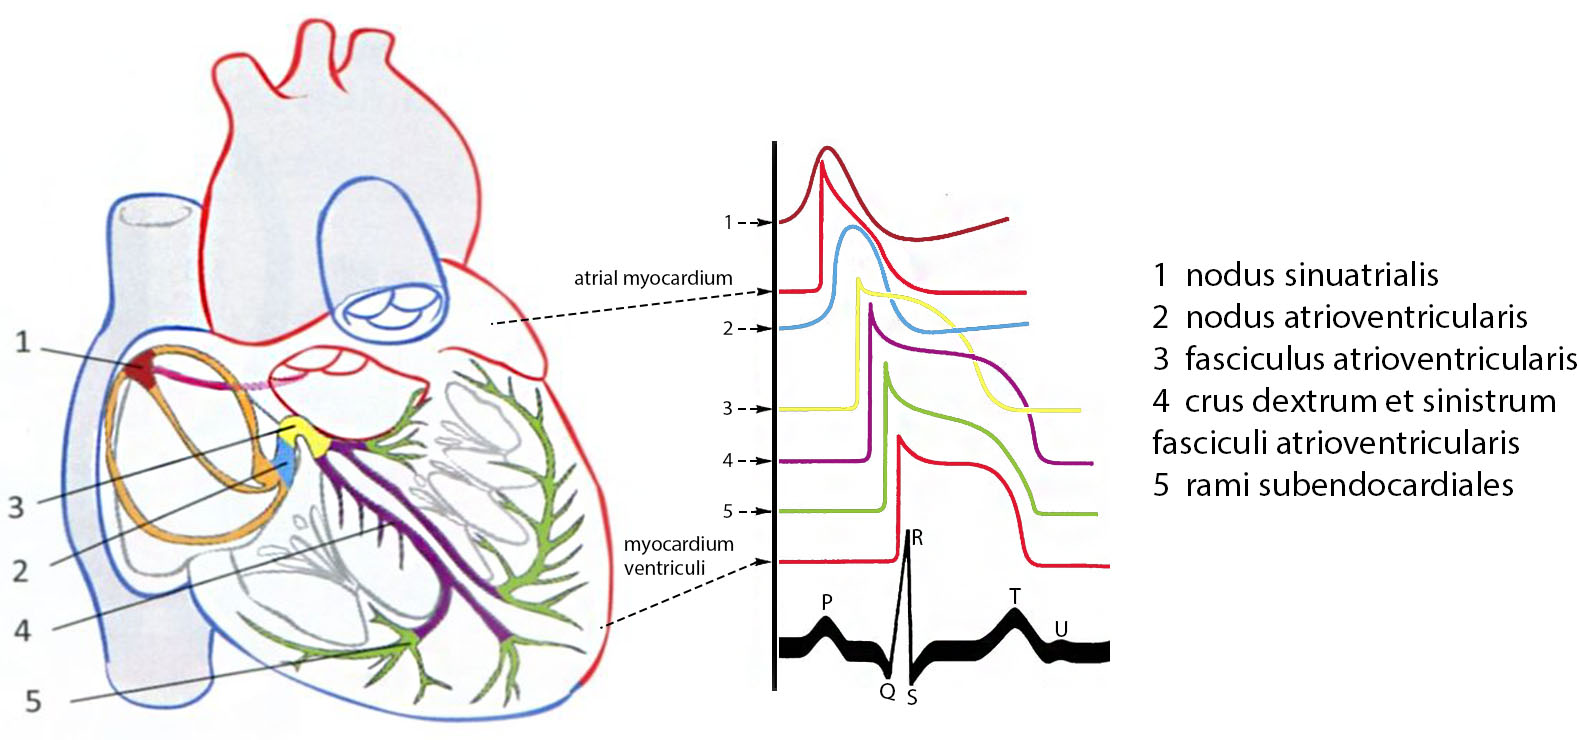
\includegraphics[width=0.9\textwidth]{../assets/anatomy/pss}
		\caption{Převodní systém srdeční (Upraveno a převzato z
			\cite{ecgpediaConduction})}
		\label{fig:pss}
	\end{center}
\end{figure}

Z funkčního hlediska se jedná o soubor specializovaných částí myokardu. První
část tvoří buňky pracovního myokardu, jejichž hlavním úkolem je kontrakce
\cite{Cihak2016}. Druhou část reprezentují specializované buňky převodního
srdečního systému --- kardiomyocyty --- které jsou morfologicky těžko
odlišitelné, avšak funkčně, na rozdíl od buněk pracovního myokardu mají na
starosti autonomní generaci akčního potenciálu (AP) a rychlé vedení vzruchu
elektrického charakteru za účelem podráždění myokardu (excitabilita) a vyvolání
jeho stahu (systola). Ke vzniku těchto vzruchů dochází uvnitř orgánu (automacie)
a poté se šíří dále. Navzájem jsou propojeny interkalárními disky (disci
intercalares), které vznikají spojením koncových cytoplazmatických výběžků
kardiomyocytů a tvoří tak komplexní síť, sloužící k vedení těchto vzruchů. V
místech, kde toto propojení nevzniká jsou spoje mezi jednotlivými buňkami
zajištěny desmozomy a nexy umožňující jejich vzájemnou komunikaci
\cite{Dylevsky2013, Stejfa2006}.

Srdce, konkrétně srdeční svalovinu (myokard) spolu s PSS, je tedy možné
charakterizovat několika hlavními funkcemi \cite{Stejfa2006}:
\begin{itemize}
	\item \textit{Automacie (chronotropie, samočinnost)} --- samočinná rytmická
	      generace elektrických impulzů pacemakerovými buňkami k podnícení
	      pravidelné kontrakce.
	\item \textit{Excitabilita (bathmotropie, dráždivost)} --- reakce na
	      podráždění elektrickým impulzem depolarizací.
	\item \textit{Konduktivita (dromotropie, vodivost)} --- vedení vzniklých
	      elektrických vzruchů celou srdeční svalovinou.
	\item \textit{Stážlivost (inotropie, kontraktilita)} --- mechanická odpověď
	      kontraktilních buněk pracovního myokardu na vzniklé elektrické
	      podněty.
\end{itemize}

V zmíněných dvou funkčních částech je také potřeba rozlišovat rozdíly na buněčné
úrovní, a to konkrétně v rámci membránových potenciálů.

Buňky pracovního myokardu sice nemají schopnost samovolně vytvářet vzruchy ale
jejich dráždění vyvolává šíření akčního potenciálu napříč myokardem, což má za
následek zahájení kontrakce. Jejich klidový membránový potenciál se pohybuje
okolo -90 mV. Změnou klidového membránového potenciálu vzniká akční potenciál,
jehož časový průběh sestává z následujících fázi: rychlá depolarizace (fáze 0),
časná repolarizace (fáze 1), plató akčního potenciálu (fáze 2), konečná
repolarizace (fáze 3) a návrat ke klidovému potenciálu (fáze 4)
\cite{Petrek2019}.

\begin{figure}[h]
	\centering
	\begin{subfigure}{0.4\textwidth}
		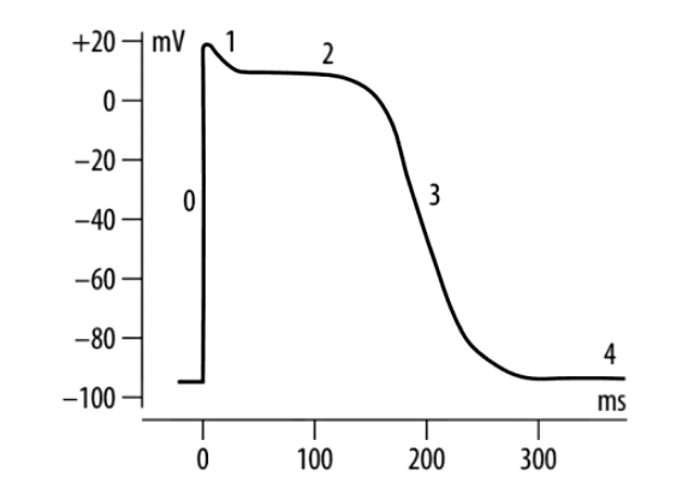
\includegraphics[width=1\textwidth]{../assets/anatomy/myokard_ap}
		\caption{Akční potenciál buňky pracovního myokardu \cite{Petrek2019}}
		\label{fig:myokard_ap}
	\end{subfigure}
	\hfil
	\begin{subfigure}{0.5\textwidth}
		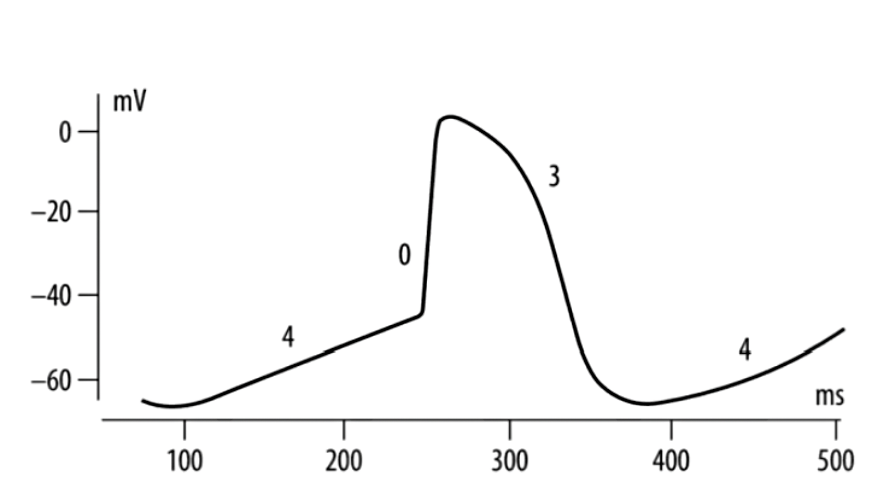
\includegraphics[width=1\textwidth]{../assets/anatomy/pss_ap}
		\caption{Akční potenciál buňky převodního systému srdce
			\cite{Petrek2019}}
		\label{fig:pss_ap}
	\end{subfigure}
	\caption{Rozdíl průběhů akčních potenciálu pracovního myokardu a převodního
		systému srdce: 0 --- rychlá depolarizace, 1 --- časná repolarizace, 2
		--- plató akčního potenciálu, 3 --- konečná repolarizace, 4 --- návrat
		ke klidovému potenciálu}
	\label{fig:ap}
\end{figure}

Klidový membránový potenciál pacemakerových buněk --- buněk SA a AV uzlu --- je
nižší, než u buněk pracovního myokardu (-50 až -70 mV) a samovolně klesá k
prahové hodnotě (spontánní diastolická depolarizace). Jakmile klidový potenciál
dosáhne prahové hodnoty vzniká další akční potenciál. Průběh akčního potenciálu
se od buněk pracovního myokardu také liší. Chybí zde 1. a 2. fáze. Přehledněji
je možné pozorovat rozdíly porovnáním křivek AP na Obr. \ref{fig:ap}
\cite{Petrek2019}.

Elektrické vzruchy, vyvolávající rytmické smršťování srdečního svalu, primárně
vznikají v SA uzlu, uloženém při ústí horní duté žíly, ve stěně pravé síně.
Tento uzel je udavatel srdečního rytmu (HR) neboli primární pacemaker a vzruchy se z
něj šíří dále systémem. Než jsou tyto impulzy převedeny přes Hisův svazek na
Purkyňova vlákna, prochází vzruch AV uzlem (sekundární pacemaker), kde dochází k
jeho zpomalení a tvorbě časové prodlevy, což má za následek postupné kontrakce
síní a komor neboli posloupnost systol a diastol. Spojení mezi SA uzlem a AV
uzlem je realizováno internodálními síňovými spoji, což jsou vlákna stejného
charakteru jako u PSS. Tyto spoje umožňují rozvádět vzruchy z SA uzlu rychleji
než samotná svalovina síní a excitovat tak AV uzlík v krátkých intervalech.
Vzruchy je pak možno mezí síněmi a komorami vést pomalu či rychleji, což
představuje jeden z regulačních mechanismů srdeční frekvence
\cite{Dylevsky2013,Cihak2016}.

Tento sled, pravidelnost srdečního rytmu a proměnlivost srdečních akcí vůči
změnám v organismu, zajišťuje několikastupňový regulační systém. Zachycením
těchto elektrických proudů v čase spolu se změnami jejich potenciálu vzniká tzv.
elektrokardiogram (EKG), na kterém je možné pozorovat průběh elektrického
srdečního cyklu s jeho jednotlivými fázemi (Obr. \ref{fig:pss} --- P, Q, R, S,
T, U) \cite{Dylevsky2013,Cihak2016}.


\subsubsection{Regulace srdeční frekvence}
\label{section:hr_regulation}
Změny v srdeční frekvenci (chronotropie) a její variabilitě jsou jedním z
následků regulace srdeční činnosti, která mimo jiné ovliňuje také inotropii,
dromotropii a bathmotropii. Regulaci dělíme na dvě úrovně v závislosti na místě
průběhu regulačního děje, a to na intrakardiální a extrakardiální.
Intrakardiální regulační děje probíhají v srdci samotném, například následkem
mechanických změn myokardu. Blíže tyto děje popisuje například Starlingův zákon
nebo Bainbridgeův reflex \cite{Kittnar2020}. Extrakardiální děje se dělí dále na
nervové a humorální. Jelikož je srdeční frekvence řízena hlavně nervově, tak se
tato kapitole věnuje podrobněji extrakardiálním vlivům \cite{Orel2019}.

\paragraph*{\textit{Nervová regulace srdečního rytmu}\\} Srdce je inervováno
autonomním (vegetativním) nervovým systémem, konkrétně pregangliovými
parasympatickými vlákny (rami cardiaci nervi vagi) z bloudivého nervu (nervus
vagus) a sympatickými vlákny z krčního kmene sympatiku (n. cardiacus cervicalis
superior, medius et inferior), společně s větvemi jeho horního hrudního úseku
(nn. cardiaci thoracici) \cite{Dylevsky2013,Kittnar2020}. Tato vlákna realizují
regulační děje, vzniklé na úrovní prodloužené míchy (medulla oblongata) v
kardioexcitačním nebo kardioinhibičním centru. Inervace tohoto typu představují
jeden z vyšších stupňů regulačních mechanismů a jejich dráždění má vliv na
srdeční frekvenci a její variabilitu \cite{Dylevsky2013,Trojan2002}.

\begin{figure}[h]
	\begin{center}
		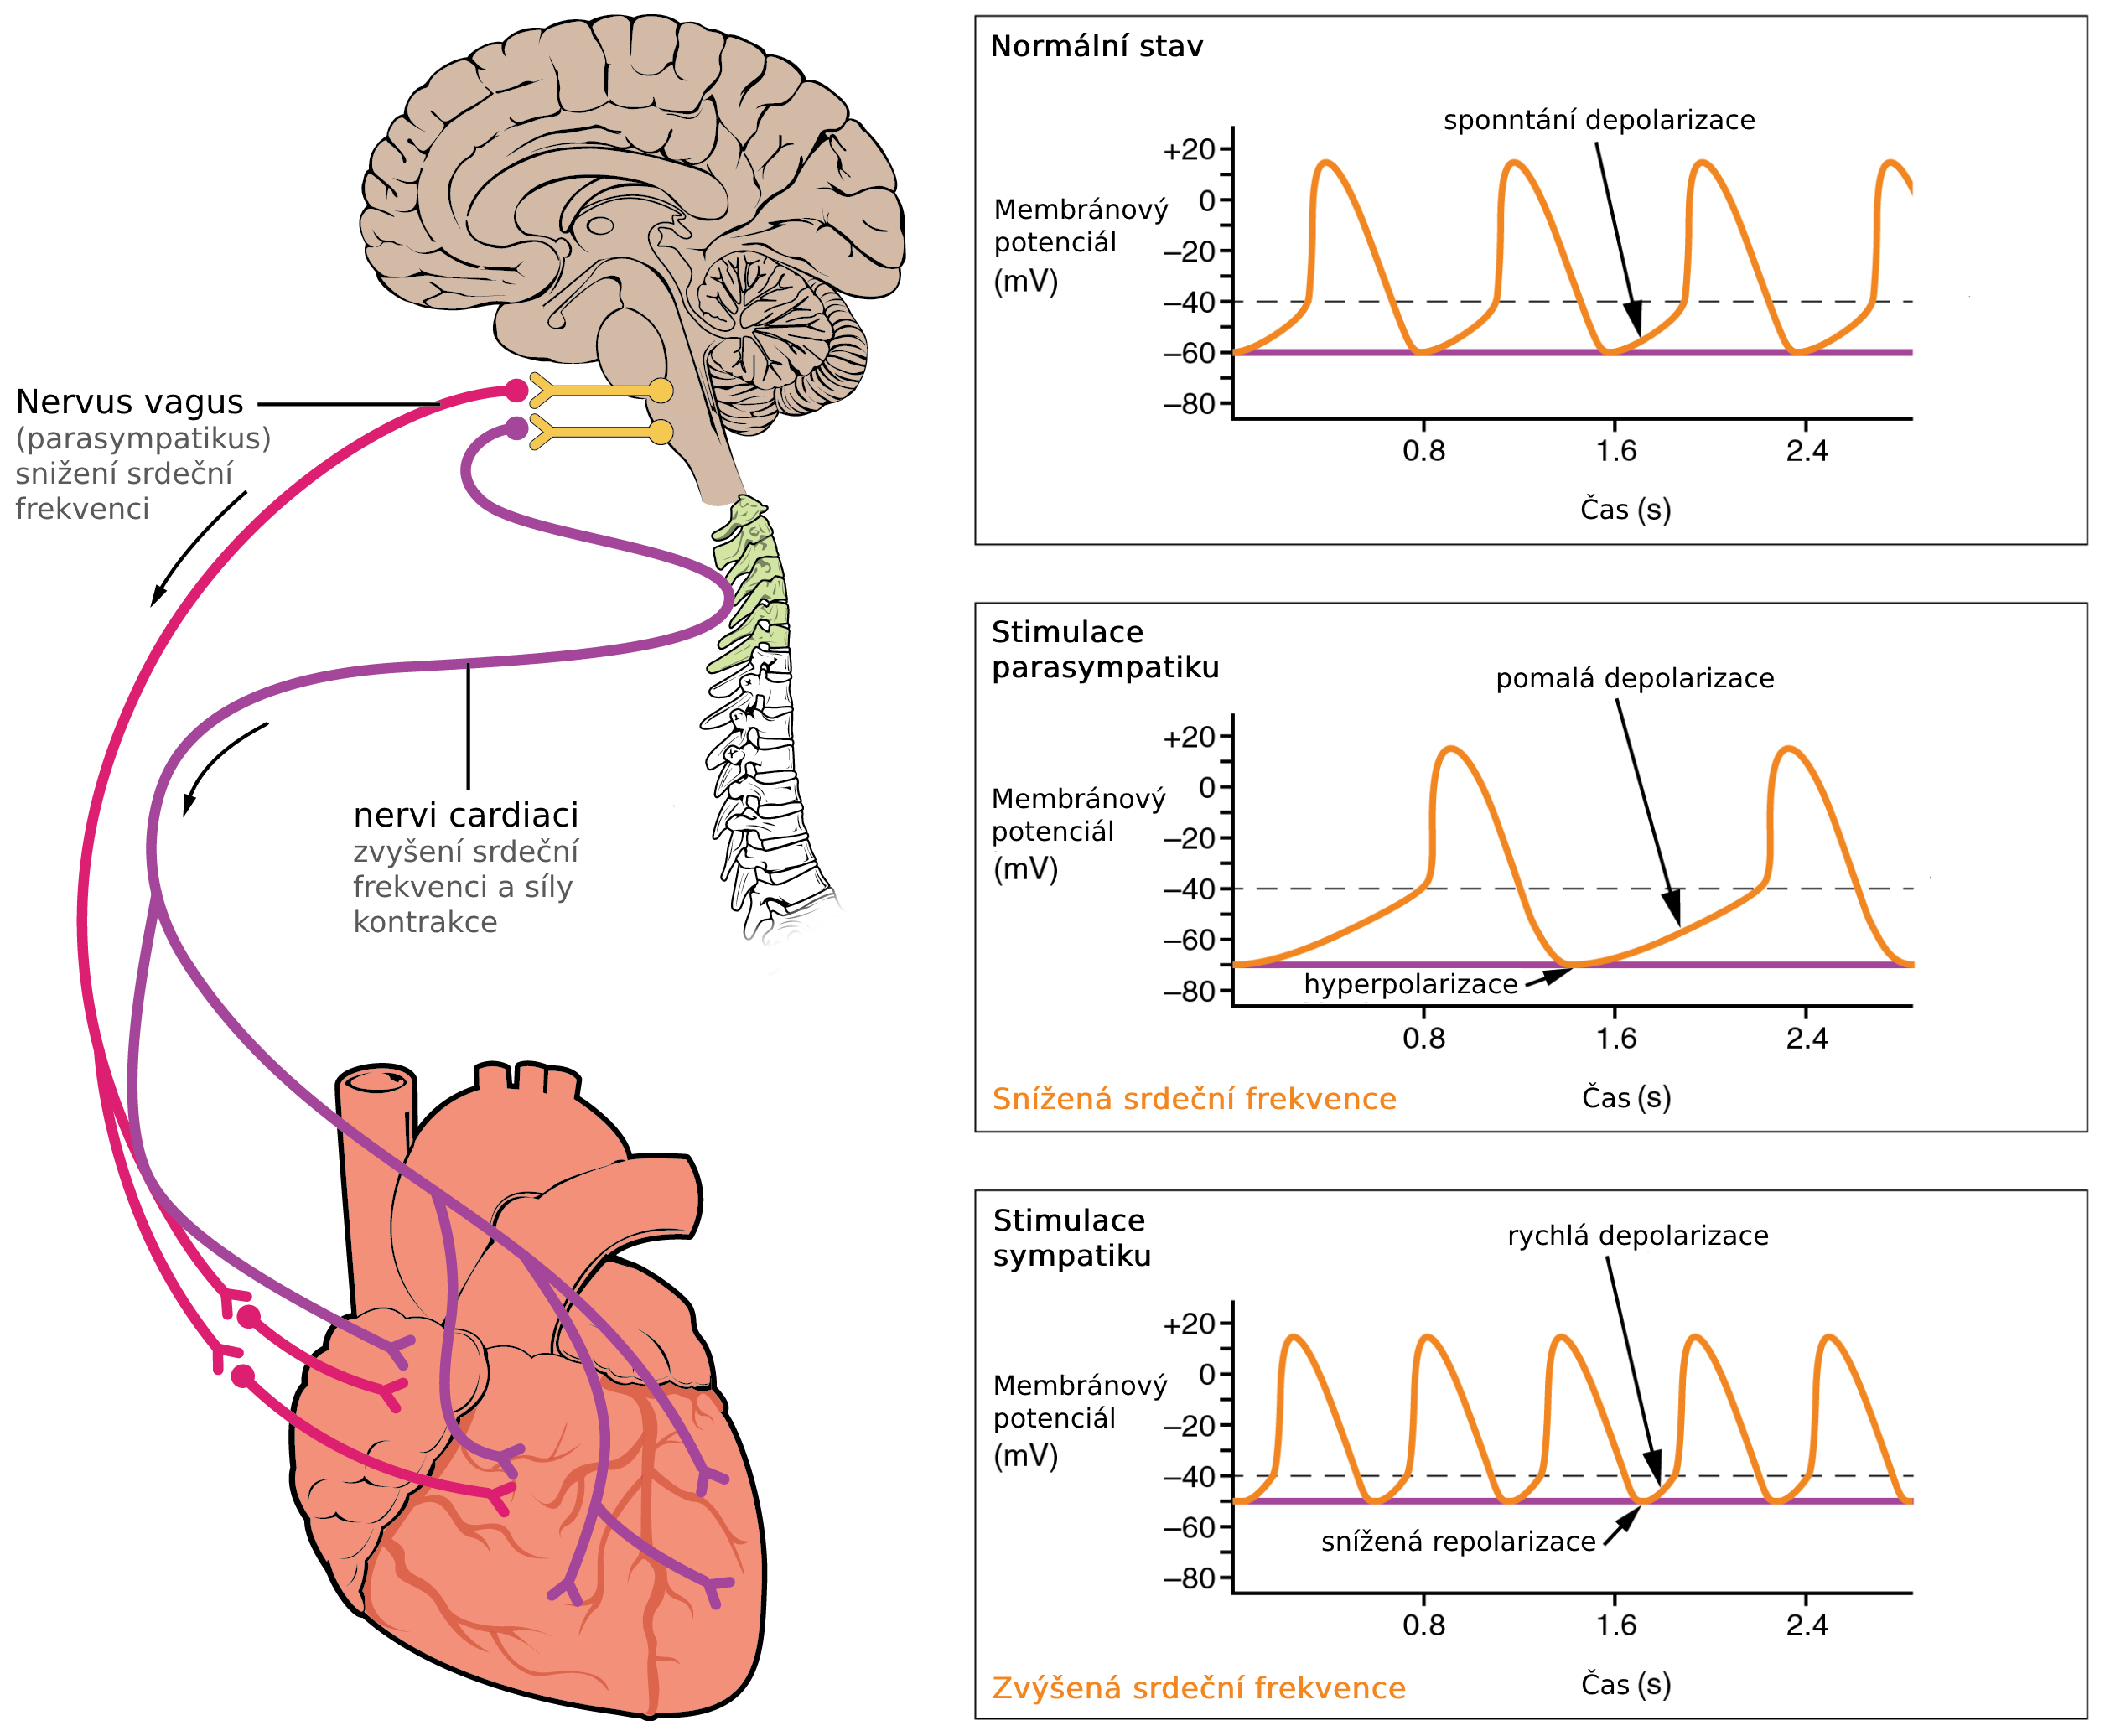
\includegraphics[width=1\textwidth]{../assets/anatomy/hr_regulation}
		\caption{Autonomní invervace kardioexcitačních a kardioinhibičních
			oblastí nacházejících se v prodloužené míše a jejich vliv na
			normální sinusový rytmus (Upraveno a převzato z \cite{OpenStax})}
		\label{fig:hr_regulation}
	\end{center}
\end{figure}

Srdeční odezva na tyto nervové podněty je realizována na nejnižší intrakardiální
úrovní pomocí srdečních ganglií, které se skládají z neuronů. Přesněji jsou to
hlavně cholingerní (vagální) a adrenergní (sympatické) srdeční neurony, sloužící
jako vagální spínací body se schopností reakce na chemické, mechanické a
elektrofyziologické podněty. Díky tomu může například nervová aktivita v
prefrontální kůře modulovat HRV (\ref{section:hrv}). Blíže tyto vztahy popisuje
model Neuroviscerální integrace (NVI) \cite{Smith2017}.

Vliv parasympatiku je realizován uvolňováním mediátoru --- acetylcholinu --- z
koncových postgangliových vláken. Odpověď probíha v srdeční tkání díky
muskarinovým cholingerním recepotorům. Stimulací těchto receptorů se zpomaluje
proces spontánní diastolické depolarizace. To má za následek nižší srdeční
frekvenci (negativní chronotropie) v SA uzlu a zpomalení síňokomorového převodu
vzruchů v AV uzlu. Obecně tedy stimulace parasympatiku způsobuje včetně
zpomalení HR a síňokomorového převodu také snížení srdeční kontrakce a
excitability myokardu \cite{Kittnar2020}.

Stimulací sympatiku nastávají přesně opačné účinky než u parasympatiku. Ty
zahrnují zrychlení HR a síňokomorového převodu spolu se zvýšenou excitabilitou a
silou kontrakcí myokardu. Mediátorem je zde noradrenalin, který v
kardiomyocytech aktivuje \textbeta-adrenergní receptory, což vyvolává zrychlenou
spontánní depolarizaci. Výsledkem je primárně již zmíněná zvýšená srdeční
frekvence \cite{Kittnar2020}.

\paragraph*{\textit{Humorální regulace srdečního rytmu}\\} Regulace na této
úrovni vzniká vlivem hormonů, a to především působením katecholaminů ---
adrenalin a noradrenalin ---, produkovaných dření nadledvin nebo adrenergními
neurony sympatiku. Mají okamžitý nástup účinků, které jsou podobné těm jako u
stimulace sympatiku. Mezi další hormony ovlivňující srdeční frekvenci patří také
například hormony štítné žlázy, tyroxin a trijodthyronin
\cite{Kittnar2020,Orel2019}.

\paragraph*{\textit{Další faktory regulující srdeční rytmus}\\} Dalšími vlivy,
které ovlivňují srdeční frekvenci jsou například: koncentrace různých
elektrolytů v těle, tělesná teplota, rovnováha pH, dýchání, fyzická zátěž nebo
různé druhy kognitivní zátěže. Dále změny krevního tlaku, na které jsou citlivé
baroreceptory umístěné v oblouku aorty (arcus aortae) neboli tzv. reflexní
řízení. Mimo jiné se tato frekvence liší i věkem, pohlavím či zdravotními
podmínkami \cite{Kittnar2020}.

\subsection{Elektrokardiografie}
\label{section:electrocardiography}
Jednou z nejčastějších neinvazivních diagnostických metod v klinické praxi,
hlavně v oblasti kardiologie, je záznam a interpretace elektrické aktivity srdce
neboli elektrokardiografie. Princip této metody spočívá v měření elektrických
projevů srdeční aktivity na povrchu lidského těla. Každá perioda srdečního cyklu
je na buněčné úrovní doprovázená genezí nerovnoměrného elektrického napětí (AP),
což má za následek vznik místních elektrických proudů, resp. elektrického pole v
okolí myokardu \cite{Kittnar2020}. Vzniklé elektrické pole je zde ve skutečnosti
součtem jednotlivých elektrických polí každé srdeční buňky, kterou je možno
vyjádřit elementárním vektorem. Elementární vektory vyjadřují velikost a směr
elektrického pole \cite{Stejfa2006}. Sumací vektorů v jednom časovém momentu
vzniká okamžitý vektor elektrického pole jehož orientace a velikost
charakterizují výslednou naměřenou amplitudu v specifickém svodu, viditelnou na
EKG křivce \cite{Surawicz2008,Kittnar2020}.

Tkáně v lidském těle díky jejich elektrickým vlastnostem plní při styku s
elektrickým polem úlohu vodiče a díky tomu je možné mezi různými místy na
povrchu těla naměřit napětí. K snímaní napětí na rozhraní kůže se používají
elektrody. Zaznamenáváním výsledné hodnoty naměřených rozdílů potenciálu mezi
elektrodami v čase vzniká tzv. elektrokardiogram. Měření se liší počtem
použitých svodů a jejich lokalizací na lidském těle. Elektrokardiografii je tedy
možné kategorizovat z hlediska počtu, zapojení a umístění svodů do těchto
skupin: \cite{Haberl2012,Kittnar2020}:

\begin{enumerate}
	\item \textbf{Einthovenovy bipolární končetinové svody (I, II, III)} ---
	      vytváří tzv. teoretický Einthovenovův rovnoramenný trojúhelník, jehož
	      přibližným středem je srdce. Elektrody se v tomto případě většinou
	      nachází na horních končetinách a levé dolní končetině, přičemž dvě z
	      nich jsou elektrody aktivní. Měřenou amplitudu udává rozdíl potenciálu
	      aktivních elektrod. Tyto svody jsou často nazývané standardními
	      \cite{Kittnar2020}.
	      \begin{figure}[H]
		      \begin{center}
			      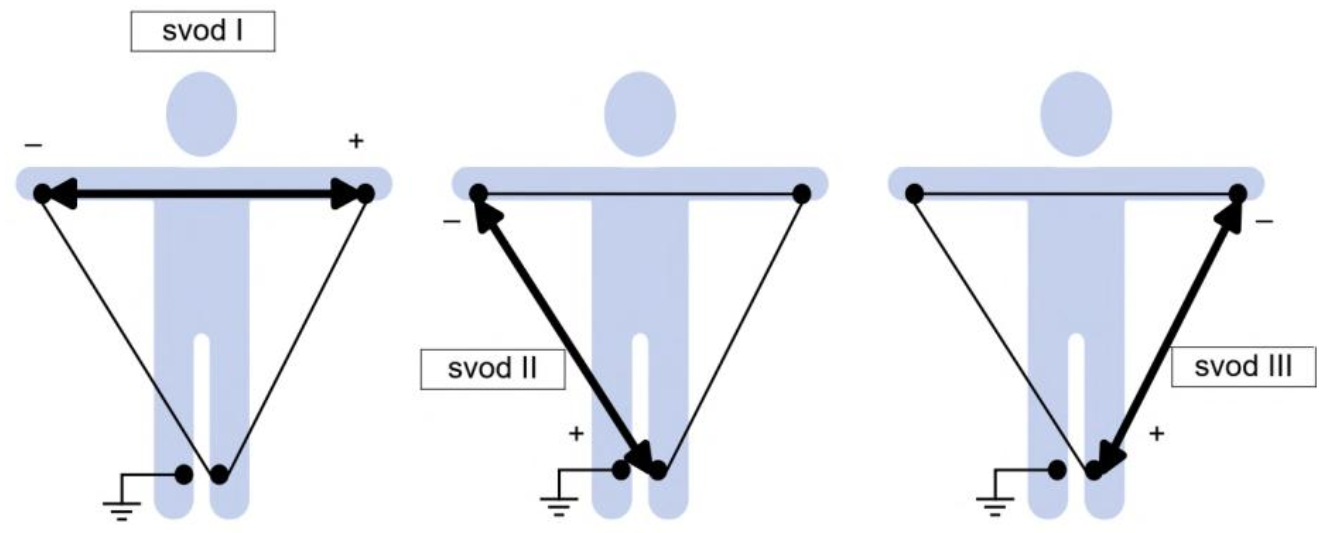
\includegraphics[width=0.75\textwidth]{../assets/anatomy/bipolar}
			      \caption{Bipolární končetinové svody \cite{Kittnar2020}}
			      \label{fig:bipolar}
		      \end{center}
	      \end{figure}
	\item \textbf{Goldbergerovy unipolární končetinové svody (aVR, aVL, aVF)}
	      --- původně tvořily spoje aktivních elektrod s Wilsonovou virtuální
	      svorkou. K Wilsonově svorce byly připojeny všechny končetinové svody
	      přes vyoský odpor ke zajištění nulového potenciálu na této svorce.
	      Pozdějí byl tento způsob upraven Goldbergerem, který touto modifikací
	      zesílil amplitudu svodů na záznamu. Zesílení vzniká odpojením aktivní
	      elektrody od Wilsonovy svorky čimž je následně měřen potenciál pouze
	      mezi odpojenou elektrodou a zbylými \cite{Kittnar2020}.
	      \begin{figure}[h]
		      \begin{center}
			      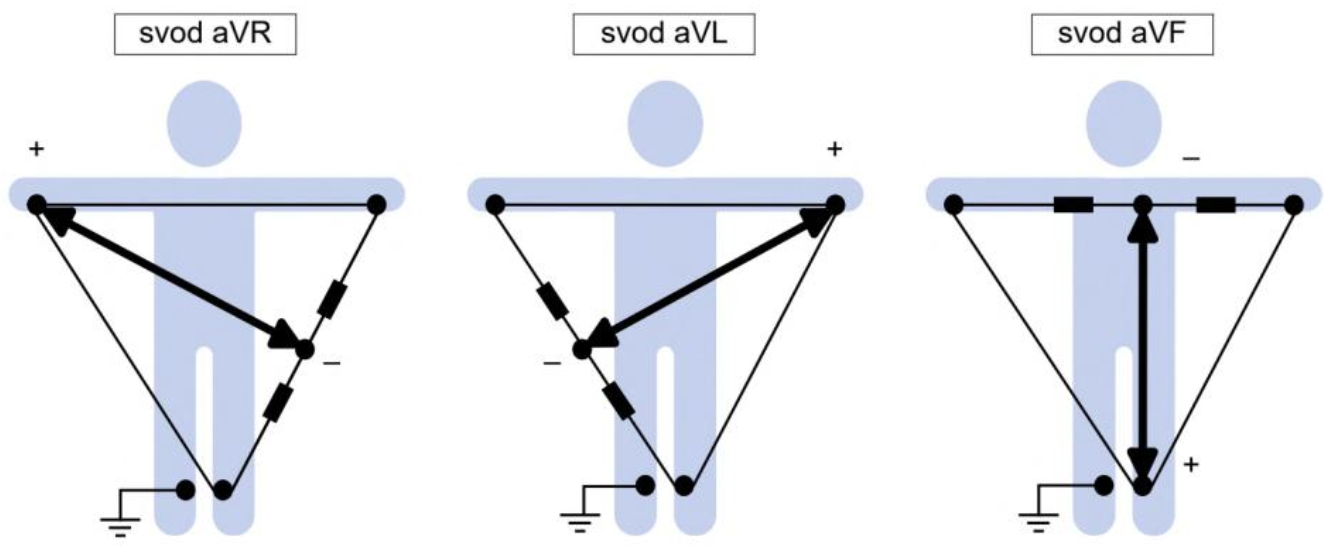
\includegraphics[width=0.75\textwidth]{../assets/anatomy/unipolar1}
			      \caption{Unipolární končetinové svody \cite{Kittnar2020}}
			      \label{fig:unipolar1}
		      \end{center}
	      \end{figure}
	\item \textbf{Wilsonovy unipolární hrudní svody (V1 -- V6)} --- sestávají z
	      šesti hrudních elektrod zapojených proti referenční Wilsonově svorce.
	      Wilsonova nulová svorka je zde opět tvořená spojením končetinových
	      svodů přes odpor. Změnou v tomto zapojení je přechod z frontální
	      roviny měření elektrické aktivity srdce do horizontální. V kombinaci s
	      předešlími Goldbergerovy svody tak vzniká prostorová informace o
	      elektrickém poli myokardu \cite{Kittnar2020}.
	      \begin{figure}[h]
		      \centering
		      \subcaptionbox{Unipolární hrudní svod \cite{Kittnar2020}}
		      [.35\linewidth]{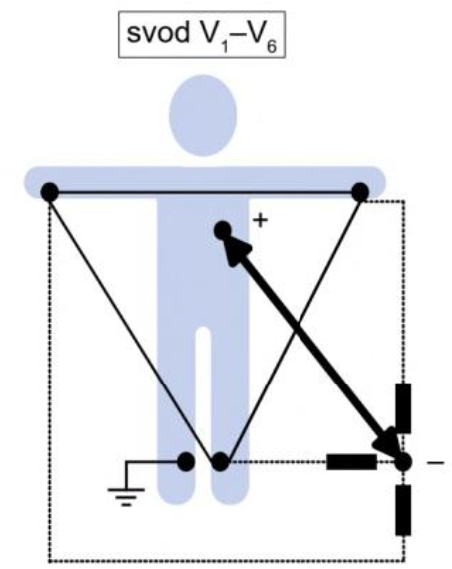
\includegraphics[height=5cm]{../assets/anatomy/unipolar2}}
		      \hfill
		      \subcaptionbox{Přiložení unipolárních hrudních svodů podle Wilsona
			      (vlevo) a přiřazení elektrod k srdci v příčném průřezu (vpravo)
			      \cite{Haberl2012}}
		      [.6\linewidth]{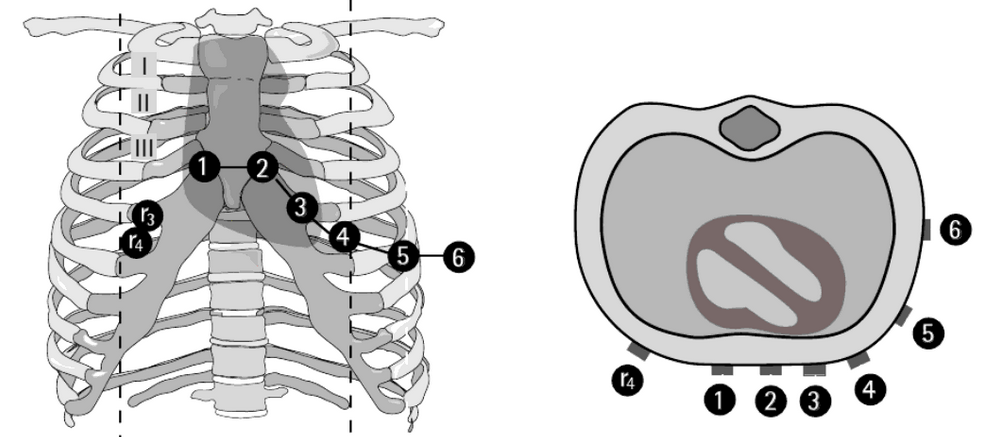
\includegraphics[height=4cm]{../assets/anatomy/unipolar3}}
		      \caption{Wilsonovy unipolární hrudní svody}
		      \label{fig:wilson}
	      \end{figure}
\end{enumerate}

Kombinací všech výše zmíněných svodů vzniká standardní klinický 12-svodový EKG
záznam, který se běžně používá v praxi. Někdy se využívají i další přídatné
svody, jako například etážové, ortogonální nebo jícnové svody. Graficky se
zaznamenává na milimetrový papír nebo je vidět na obrazovce v digitalizované
podobě. Délka záznamu se obvykle liší v závislosti na prováděné diagnostice či
terapii. K záznamu se používají různé typy EKG přístrojů, které často snímají
více biologických veličin, něž pouze elektrickou aktivitu srdce. Mezi přístroje,
které se k měření využívají, se řadí například pacientské monitory vitálních
funkcí nebo v případě mobilnějšího řešení Holterův monitor (Holter). Holterovo
monitorování se nejčastěji uplatňuje u dlouhodobého kontinuálního záznamu
srdeční aktivity, obvykle 24 hodin, kde je třeba v rámci diagnostiky sledovat
příležitostné srdeční úkazy. Největší výhodou v případě Holtru je jeho malá
konstrukce v podobě krabičky o velikosti většího mobilního telefonu což umožňuje
jeho jednoduchou přenosnost \cite{Surawicz2008}.

%//TODO: Rewrite and cite this subsection 9, 10
\subsection{Zpracování záznamu srdeční aktivity}
Monitorování či analýza EKG tvoří nepostradatelnou část v mnoha diagnostických a
terapeutických případech. Díky mobilním implementacím, pomocí kterých jsme
schopni sledovat tuto biologickou aktivitu skrze chytrá zařízení je to v
současnosti trend. Než se ale na výstupu, například v podobě displeje, objeví
EKG křivka či jiné vypočtené parametry, tak se signál musí předzpracovat, jinak
by tyto parametry byly v praxi zavádějící.

\subsubsection{Potlačení nežádoucích elementů signálu}
Nezbytným krokem v předzpracování je filtrace signálu, jelikož ho zkreslují
mnohočetné okolní a elektrofyziologické vlivy, které mohou vést k jeho nesprávné
interpretaci. Nejčastější rušivé prvky, které se projevují na signálu jsou:
síťový brum (síťový 50 \si\Hz~šum), myopotenciály, pohybové artefakty nebo
špatné umístění elektrod. \cite{Surawicz2008}. 

Sítový brum neboli elektrická interference generovaná střídavým proudem ze
zásuvky, je jedním z nejběžnějších artefaktů projevujících se u biologických
signálu. Příčinou jeho vzniku může být špatné uzemnění či chod zařízení nebo
vliv elektromagnetického rušení okolní techniky v blízkosti měřícího přístroje.
Na Obr. \ref{fig:ac_Interference} je vidět vliv střídavého proudu o
frekvenci 50 \si\Hz~na EKG signál \cite{Goldberger2017}. 

Pohybové artefakty se primárně na EKG signálu projevují kolísáním elektrické
izolinie od její nulové hodnoty jako je tomu na Obr. \ref{fig:w_baseline}.
Nevznikají však pouze pohybem pacienta ale i například manipulací měřicími
kabely, špatným kontaktem elektrod nebo vlivem dýchání pacienta
\cite{Goldberger2017}.

\begin{figure}[h]
	\begin{subfigure}[b]{0.5\linewidth}
		\centering
		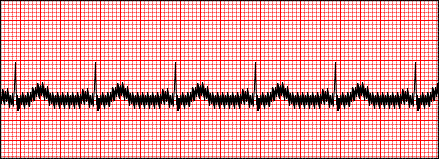
\includegraphics[width=0.8\linewidth]{../assets/ecg/ac_Interference}
		\caption{AC rušení}
		\label{fig:ac_Interference}
		\vspace{4ex}
	\end{subfigure}
	\begin{subfigure}[b]{0.5\linewidth}
		\centering
		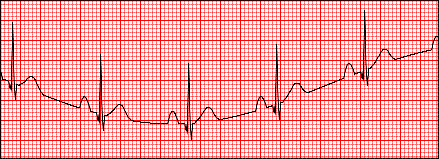
\includegraphics[width=0.8\linewidth]{../assets/ecg/w_baseline}
		\caption{Pohyb izoelektrické linie}
		\label{fig:w_baseline}
		\vspace{4ex}
	\end{subfigure}
	\begin{subfigure}[b]{0.5\linewidth}
		\centering
		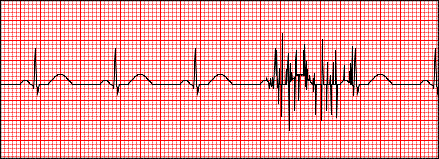
\includegraphics[width=0.8\linewidth]{../assets/ecg/muscle_tremor}
		\caption{Myopotenciály (svalový třes, tremor)}
		\label{fig:muscle_tremor}
	\end{subfigure}
	\begin{subfigure}[b]{0.5\linewidth}
		\centering
		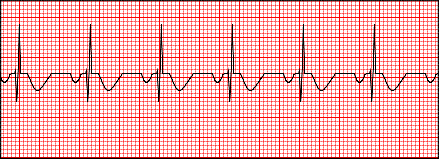
\includegraphics[width=0.8\linewidth]{../assets/ecg/rev_electrodes}
		\caption{Nesprávné umístění elektrod}
		\label{fig:rev_electrodes}
	\end{subfigure}
	\caption{Běžné EKG artefakty \cite{Mauvila2004}}
	\label{fig:common_artifacts}
\end{figure}

Svalové artefakty neboli myopotenciály jsou dalším častým typem rušení
vysokofrekvenčního charakteru, které lze pozorovat u EKG signálu. Svým způsobem
lze tento typ rušení z části řadit mezi předešlé pohybové artefakty, jelikož
mohou vznikat pohybem pacienta. Tento pohyb může být nedobrovolný například u
osob trpících Parkinsonovou chorobou, kterou obvykle doprovází svalový třes
(tremor) nebo pulzace arteriální tepny pod elektrodou \cite{Surawicz2008}.
Vlivem pohybů kosterního svalstva vzniká svalová elektrická aktivita (EMG),
která náhodně interferuje s EKG signálem. Na Obr. \ref{fig:muscle_tremor} je
vidět tato interference v podobě překrytí QRS komplexu myopotenciálem
\cite{Goldberger2017}.

V neposlední řadě, spíše než rušení, je častou chybou při záznamu EKG špatné
umístění nebo prohození elektrod. Proto je nutné pamatovat si význam barev
elektrod. Každá barva označuje specifické místo na těle, kam má být elektroda
připevněna. Pokud dojde k prohození, dochází k měření jiného chybného
potenciálu. Na Obr. \ref{fig:rev_electrodes} je vidět situace, kdy došlo k
záměně bíle a červené elektrody. Výsledkem je inverze všech vln EKG křivky (P,
Q, R, S, T) \cite{Goldberger2017,Surawicz2008}.

Filtrace nežádoucích prvků se zpravidla provádí kombinací filtrů typu horní a
dolní propust, a to jak hardwarově, například v podobě RLC obvodů, tak i
výpočetně. Výpočetní část tvoří především matematické aplikace diskrétních
lineárních a nelineárních filtrů či algoritmů kombinující více metod nebo jejich
částí. Dnes se často využívá neuronových sítí, vlnkových transformací a jiných
algoritmů někdy ve spojení s umělou inteligencí. Záleží na charakteristice
signálu a typu následné analýzy. Hlavním cílem často bývá identifikace a
segmentace jednotlivých komponentů QRS komplexu nebo extrakce specifických
složek z frekvenčního spektra signálu. Pokud je předzpracování dostatečně
efektivní a je možné tyto složky úspěšně extrahovat, aplikují se na tyto
komponenty další postupy, díky kterým jsme schopni hodnotit a analyzovat další
fyziologické jevy mezi které nejčastěji patří variabilita srdečního rytmu.

\subsubsection{Vybrané metody zpracování a extrakce komponentů}
\subsubsection{Rozdíly mezi offline a online zpracováním signálu}

%//TODO: Rewrite and cite this subsection 9, 10
\subsection{Variabilita srdeční frekvence}
\label{section:hrv}

\subsubsection{Metody hodnocení HRV}
Nejčastější a základní neinvazivní metody hodnocení HRV lze sjednotit do časové
a frekvenční oblasti ale existují i další geomterické a nelineární postupy.
Nejzákladnější běžná metoda je spektrální analýza variability srdečního rytmu,
která nám umožňuje zaznamenat a deklarovat vlivy kardiálního autonomního
nervového systému (ANS). Další využívanou metodou je akcelerovaná
fotopletysmografie (APG), kde vyšetřované místo vystavíme světelným paprskům,
které procházejí tkání a jejich odezva je pak zpracována do podoby pulsových vln
vynesených na křivce. Tyto metody jsou pak v praxi využitelné pro včasné
odhalení kardiovaskulárních onemocnění, nicméně jsou použitelné pouze ve
specifických laboratorních podmínkách a jako jiné jsou ovlivnitelné právě
fyzickými a psychologickými faktory \cite{[2, 4, 5]}. Parametry HRV můžou
sloužit pro predikci kognitivní zátěže, ale pro jejich spolehlivé určení je
nezbytný pečlivý výběr vhodných metod předzpracování signálu \cite{[1, 3]}.
Pokud bychom byli schopni hodnotit změny a vlivy kognitivní zátěže a spojit tyto
výsledky s dosavadními metodami, které hodnotí zbylé vlivy a faktory, můžeme
díky jedné metrice efektivněji určit a předpovědět zdravotní stav pacienta a
jeho potencionální změny.

\subsubsection{Korelace kvantitativních parametrů HRV s fyziologickými veličinami}


\subsubsection{Model neuroviscerální integrace}
Tento neustále doplňující se model, popisuje vztahy v rámci periferní
psychofyziologie, neurověd a autonomních funkci spjatých s regulací vagálního
tonu. Tyto znalosti a vztahy jsou kombinovány do několika detailně popsaných
teoretických vrstev, dohromady tvořících jediný framework sloužící také jako
prediktivní model, který pak usnadňuje vyhodnotit souvislosti a důsledky
zásadních fyziologických změn srdeční aktivity či veličin s ní spojených.

Tyto souvislosti mají například za následek, že odlišné druhy kognitivní zátěže
se promítají do frekvenčních domén. Specificky se projevují jako velmi nízko,
nízko a vysoko frekvenční komponenty (VLF, LF, HF), které spolu s jejich
vzájemnými poměry slouží pří samotné analýze jako indikátory činnosti
vegetativní nervové soustavy (VNS). Aby bylo ale možné tyto komponenty získat a
porovnávat či jakkoliv hodnotit srdeční aktivitu, musí se záznam srdeční
aktivity patřičně zpracovat.

\subsubsection{Praktické aplikace HRV v diagnostice a terapii}
